\chapter{Описание эксперимента}\label{chapt2}

Для модернизации существующих и создания новых рабочих органов предлагается использовать дисковый режущий инструмент, что позволяет снизить энергоёмкость и увеличить производительность. Основным контролируемым параметром, при оснащении рабочих органов уборочных машин дисковыми резцами, является сила сопротивления прочных СЛО резанию. Для более объективного изучения процесса взаимодействия дискового инструмента с прочными СЛО предлагается контролировать три составляющие силы резания: горизонтальную, боковую и вертикальную. Контроль составляющих непосредственно на рабочем органе требует больших трудозатрат, так как физические свойства (прочность, плотность, наличие абразивного материала) прочных СЛО на дорожных покрытиях постоянно меняются и зависят от: температуры окружающей среды, влажности, теплозапаса дорожного полотна и других фактором \todo{[ссылка]}, и дорогостоящего оборудования (датчики силы, оснастка для их монтажа). Опираясь на опыт работ по резанию мерзлых грунтов различными инструментами \todo{[ссылки]}, целесообразно исследовать в лабораторных условиях одиночный полноразмерный дисковый резец.

Целью проведения экспериментальных лабораторных исследований является выявления рационального радиуса закругления рабочей кромки дискового резца, а также оценки влияния шага резания, совместно с радиусом закругления рабочей кромки, на силовые показатели процесса разрушения прочных СЛО дисковым режущим инструментом.

\section{Условия проведения эксперимента}\label{sect2_1}

При проведении экспериментальных исследований использовались дисковые резцы с различным радиусом закругления рабочей кромки. Радиусы закругления составляли $R=[0,5\ 1,5\ 2,5\ 3,5\ 4,5]$ мм.
Остальные параметры приняты следующие: 
\begin{itemize}
	\item диаметр дискового резца $D=200$ мм.;
	\item величина заострения дискового резца $\delta=30^\circ$;
	\item глубина резания $h=60$ мм.;
	\item шаг резания $t=[10\ 20\ 30\ 40\ 50]$ мм.;
	\item задний угол $\gamma=3^\circ\div5^\circ$;
	\item температура окружающего воздуха $-$2~$\div\ -$7~${}^\circ$С;
	\item скорость резания $0,51\ \slantfrac{\text{м}}{\text{м}}$ ($1,84\ \slantfrac{\text{км}}{\text{ч}}$).
\end{itemize}
Применение таких параметров обуславливается раннее выполненными работами по данной тематике. \todo{добавить ссылок} На рисунке \ref{img:DirForse} приведено направление действия составляющих силы сопротивления резанию и способ установки дискового инструмента относительно разрушаемого массива.
\begin{figure} [htbp]
	\center
	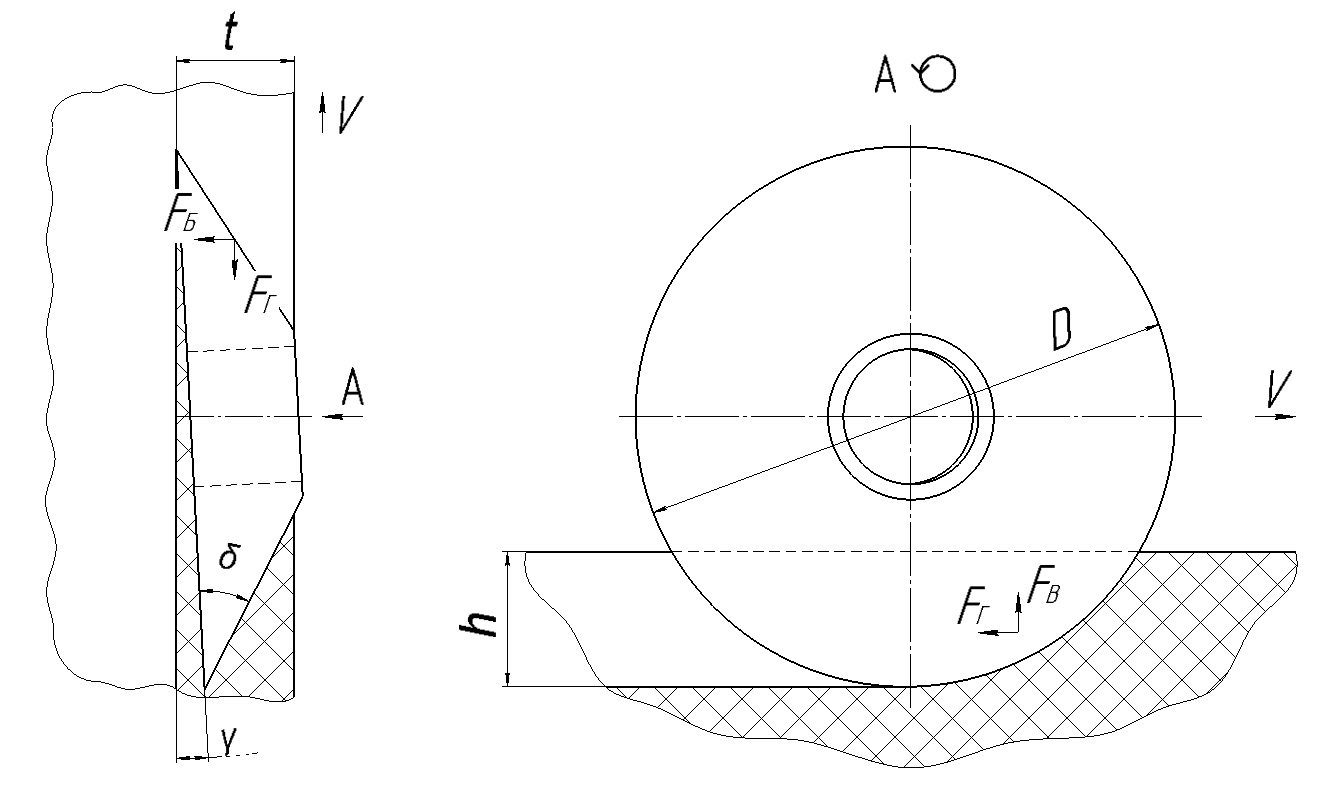
\includegraphics[width=1\textwidth]{DirForse}
	$t$ "--- шаг резания; $V$ "--- направление перемещения резца; $F_\text{Б}$ "--- боковая составляющая силы сопротивления резанию; $F_\text{Г}$ "--- горизонтальна составляющая силы сопротивления резанию; $D$ "--- диаметр дискового резца; $\delta$ "--- угол заострения дискового резца; $h$ "--- глубина резания; $F_\text{В}$ "--- вертикальная составляющая силы сопротивления резанию; $\gamma$ "--- угол установки дискового резца (задний угол). 
	\caption{Схема взаимодействия дискового резца с разрушаемым массивом} 
	\label{img:DirForse}  
\end{figure}

\section{Планирование эксперимента}\label{sect2_2}

\begin{comment}
\newenvironment{myitemize}%
	{\list{}{
		%\vspace{-1.6\onelineskip}
		\setlength{\itemsep}{0mm}%
		\setlength{\parsep}{0mm}
		\setlength{\topsep}{0mm}
		\setlength{\parskip}{0mm}
		\setlength{\partopsep}{0mm}
	    \setlength{\listparindent}{0mm}
	    \setlength{\labelsep}{0cm}%
	    \setlength{\leftmargin}{7.8mm}
	    \setlength{\labelwidth}{7.8mm}
     }\item\relax}
	{\endlist}
\end{comment}
Имеется набор из пяти дисковых резцов с радиусом закругления рабочей кромки $R$ соответствующим следующему ряду: $[0,5\ 1,5\ 2,5\ 3,5\ 4,5]$ мм. Принимаем глубину резания $h=60$ мм (Максимально допустимая высота снежно-ледяных образований), шаг резания $t$ принимается равным следующему ряду: $[10\ 20\ 30\ 40\ 50]$ мм.

Имеем 2 фактора с одинаковым количеством уровней, первый фактор ($R$) 5 уровней, второй фактор ($t$) 5 уровней. Для нахождения связи выше описанных факторов с горизонтальной, боковой и вертикальной составляющими силы резания запишем следующие уравнения:
\begin{equation}
\label{eq:regresF}
\begin{alignedat}{2}
	F_\text{Г}=f(R,t),\\
	F_\text{Б}=f(R,t),\\
	F_\text{В}=f(R,t).\\
\end{alignedat}
\end{equation}

Данная формулировка соответствует математической формулировки задачи регрессионного анализа. Для проведения регрессионного анализа необходимо проведение эксперимента со всевозможными сочетаниями факторов.

Число всех возможных состояний системы:
\begin{equation}
\label{eq:allfactors}
S=\prod_{i=1}^n p_i,
\end{equation}
где $ p_i $ "--- количество уровней $i$-ого фактора; 
	$ n $ "--- количество факторов.
	
Из формулы \ref{eq:allfactors} рассчитаем минимальное количество опытов с учетом вышеизложенных априорных данных, оно будет равно 30. Однако, мы не можем считать влияние других, не учитываемых, факторов незначительным. Поэтому необходимое количество повторений каждого опыта при каждой комбинации переменных величин установим статистическим путем \cite{Zelenin}. Для этого рассчитаем величину среднего квадратичного отклонения (СКО):
\begin{equation}
\label{eq:sigma_x}
\sigma_x=\sqrt{\frac{\sum_{i=1}^n (x_i-\bar{x})^2}{n-1}},
\end{equation}
где $ x_i $ "--- результаты $ i $-го измерения;
	$ \bar{x} $ "--- среднее арифметическое ряда измерений;
	$ n $ "--- общее число опытов.

Коэффициент вариации:
\begin{equation}
\label{eq:var}
K_{\text{ВАР}}=\frac{\sigma_x}{\bar{x}}\cdot100\%
\end{equation}

Далее с помощью соотношения: $ \frac{K_{\text{ДОП}}}{K_{\text{ВАР}}} $, где $ K_{\text{ДОП}} $ "--- коэффициент допустимого отклонения (примем 12~\%, для получения надежности экспериментальных результатов), $ K_{\text{ВАР}} $ "--- коэффициент вариации, и таблицы \ref{tbl:NOpitov} определим необходимое количество повторений одного опыта



\begin{table} [htbp]%
	\centering
	\caption{Определение количества опытов с надежностью 0,95}%
	\label{tbl:NOpitov}% label всегда желательно идти после caption
	\begin{tabularx}{\textwidth}{*2{|X}||*2{X|}}
		\hline
		 $ \frac{K_{\text{ДОП}}}{K_{\text{ВАР}}} $ &  Необходимое число опытов &
		 $ \frac{K_{\text{ДОП}}}{K_{\text{ВАР}}} $ &  Необходимое число опытов  \tabularnewline
		\hline
		\hline
		2,000	& 1	& 0,591	& 11 \tabularnewline
		1,389	& 2	& 0,568	& 12 \tabularnewline
		1,132	& 3	& 0,544	& 13 \tabularnewline
		0,980	& 4	& 0,524	& 14 \tabularnewline
		0,876	& 5	& 0,506	& 15 \tabularnewline
		0,800	& 6	& 0,490	& 16 \tabularnewline
		0,741	& 7	& 0,475	& 17 \tabularnewline
		0,693	& 8	& 0,462	& 18 \tabularnewline
		0,653	& 9	& 0,450	& 19 \tabularnewline
		0,620	& 10& 0,438	& 20 \tabularnewline
		\hline
	\end{tabularx}%
\end{table}

Для уточнения числа опытов при каждой комбинации факторов следует предварительно провести 20 опытов при неизменных параметрах режима резания.

\section{Механизированный лабораторный стенд}\label{sect2_3}

\begin{figure} [htbp]
	\center
	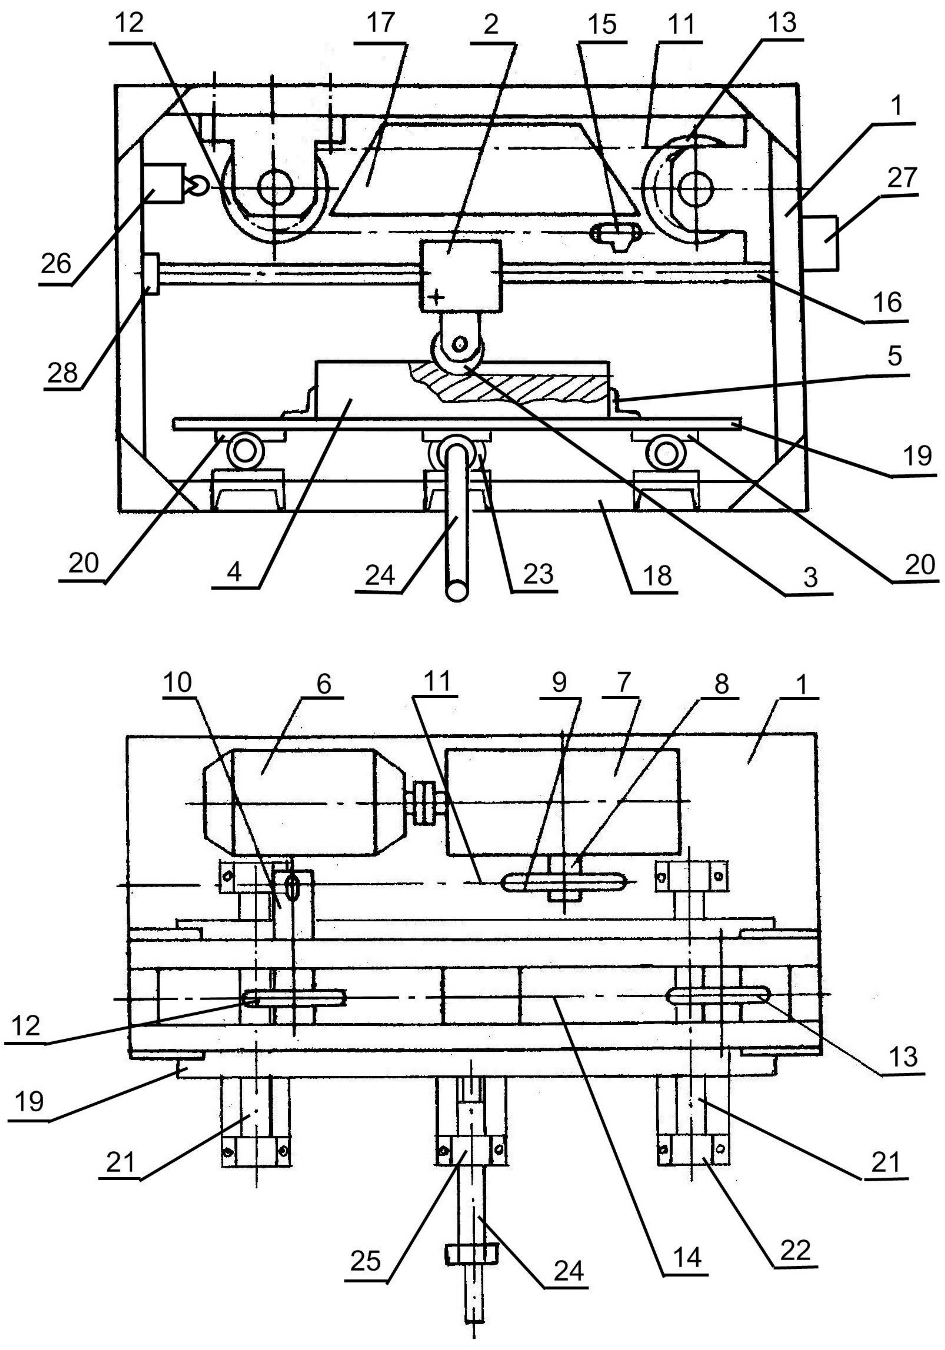
\includegraphics[scale=0.35]{Stend}
	
	1 "--- опорная рама; 2 "--- тензометрическая головка; 3 "--- режущий инструмент; 4 - образец льда; 5 "--- упоры; 6 "--- электрический двигатель; 7 "--- редуктор; 8 "--- выходной вал редуктора; 9 "--- приводная звездочка; 10 "--- ведущий вал цепной передачи; 11 "--- цепь; 12, 13 "--- звездочки тяговой цепи; 14 "--- тяговая цепь привода; 15 "--- захват; 16 "--- направляющие тензометрической головки; 17 "--- шина; 18 "--- нижняя балка рамы; 19 "--- несущая плита; 20 "--- подшипники скольжения; 21 "--- направляющие механизма поперечной подачи образца; 22 "--- опоры; 23 "--- ходовой механизм; 24 "--- поворотная рукоятка; 25 "--- опора поворотной рукоятки, 26 "--- конечный выключатель; 27 "--- кнопочная станция; 28 "--- демпферы.
	\caption{Схема лабораторного стенда} 
	\label{img:Stend}  
\end{figure}

Стенд содержит опорную раму 1 сварной конструкции, на которой смонтированы две цилиндрические направляющие 16, по которым перемещается тензометрическое звено 2 с закрепленным на нем режущим инструментом 3. На нижней балке 18 опорной рамы 1 стенда смонтирован механизм поперечной подачи образца 4 льда, включающий несущую плиту 19, к нижней поверхности которой, основанием вверх, прикреплены четыре подшипника скольжения 20, которые попарно сопряжены с двумя параллельными цилиндрическими направляющими 21, с возможностью продольного перемещения по ним. Концы направляющих 21 жестко закреплены в опорах 22, смонтированных на нижней балке 18 опорной рамы 1 стенда. В средней части несущей плиты 19, на ее нижней поверхности, установлен ходовой механизм 23, выполненный в виде втулки, на внутренней поверхности которой выполнена ходовая резьба.
 
С резьбой ходового механизма взаимодействует резьбовая часть поворотной рукоятки 24, цилиндрическая часть которой установлена в опоре 25 нижней части опорной рамы 1, с возможностью вращения в ней и без передвижения в осевом направлении. Образец льда 4 устанавливается на верхней поверхности несущей плиты 19 и жестко фиксируется упорами 5.

\begin{figure} [h]
	\center
	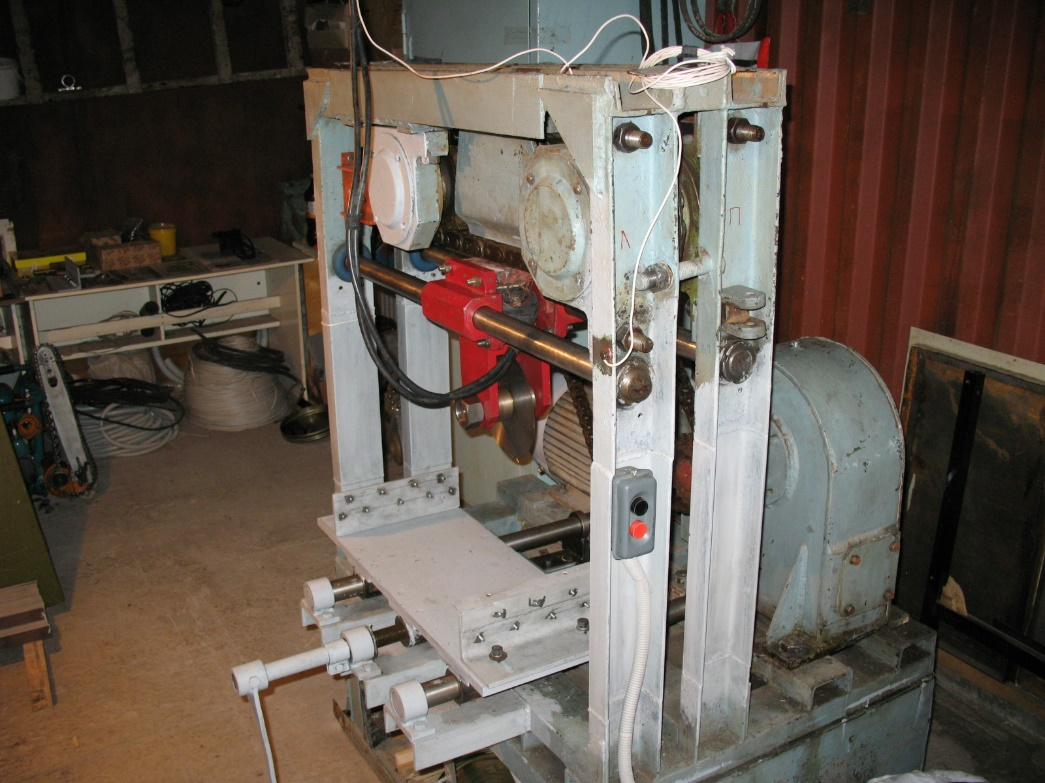
\includegraphics[width=\textwidth]{StendFoto}
	\caption{Внешний вид стенда для исследования процесса резания льда} 
	\label{img:StendFoto}  
\end{figure}

Привод тензометрической головки 2 включает электрический двигатель 6, червячный редуктор 7 с выходным валом 8, на котором закреплена звездочка 9 связанная со звездочкой ведущего вала 10 цепью 11, ведущую и ведомую звездочки 12, 13 тяговой цепи 14 привода. На одном из звеньев цепи 14 закреплен захват 15, при помощи которого, осуществляется перемещение тензометрической головки 2, по направляющим 16. Для предотвращения прогиба тяговой цепи 14 на опорной раме 1 установлена шина 17.

Управление электродвигателем 6 привода тензометрической головки 2 стенда осуществляется кнопочной станцией 27. Для автоматического отключения двигателя от электрической сети после проведения реза, на левой вертикальной опоре стенда установлен конечный выключатель 26. Окончательная остановка тензометрической головки в крайнем левом положении при резании на большой глубине, производится демпферами 28. Регулировка глубины резания, осуществляется с помощью калиброванных прокладок (на рисунках не показаны) и установкой режущего инструмента различной геометрической формы.

\section{Аппаратно-программный измерительный комплекс}\label{sect2_4}

Для контроля составляющих силы сопротивления прочных СЛО резанию необходимо спроектировать измерительный комплекс. Наиболее широкое распространение, для измерения различных сил резания, получил тензометрический метод контроля \todo{[ссылки]}. Он заключает в себе простоту и дешевизну измерений без потери точности измерений. Задача контроля силы сопротивления прочных СЛО резанию сводится к контролю электрического сопротивления чувствительных элементов.

\begin{figure} [htbp]
	\center
	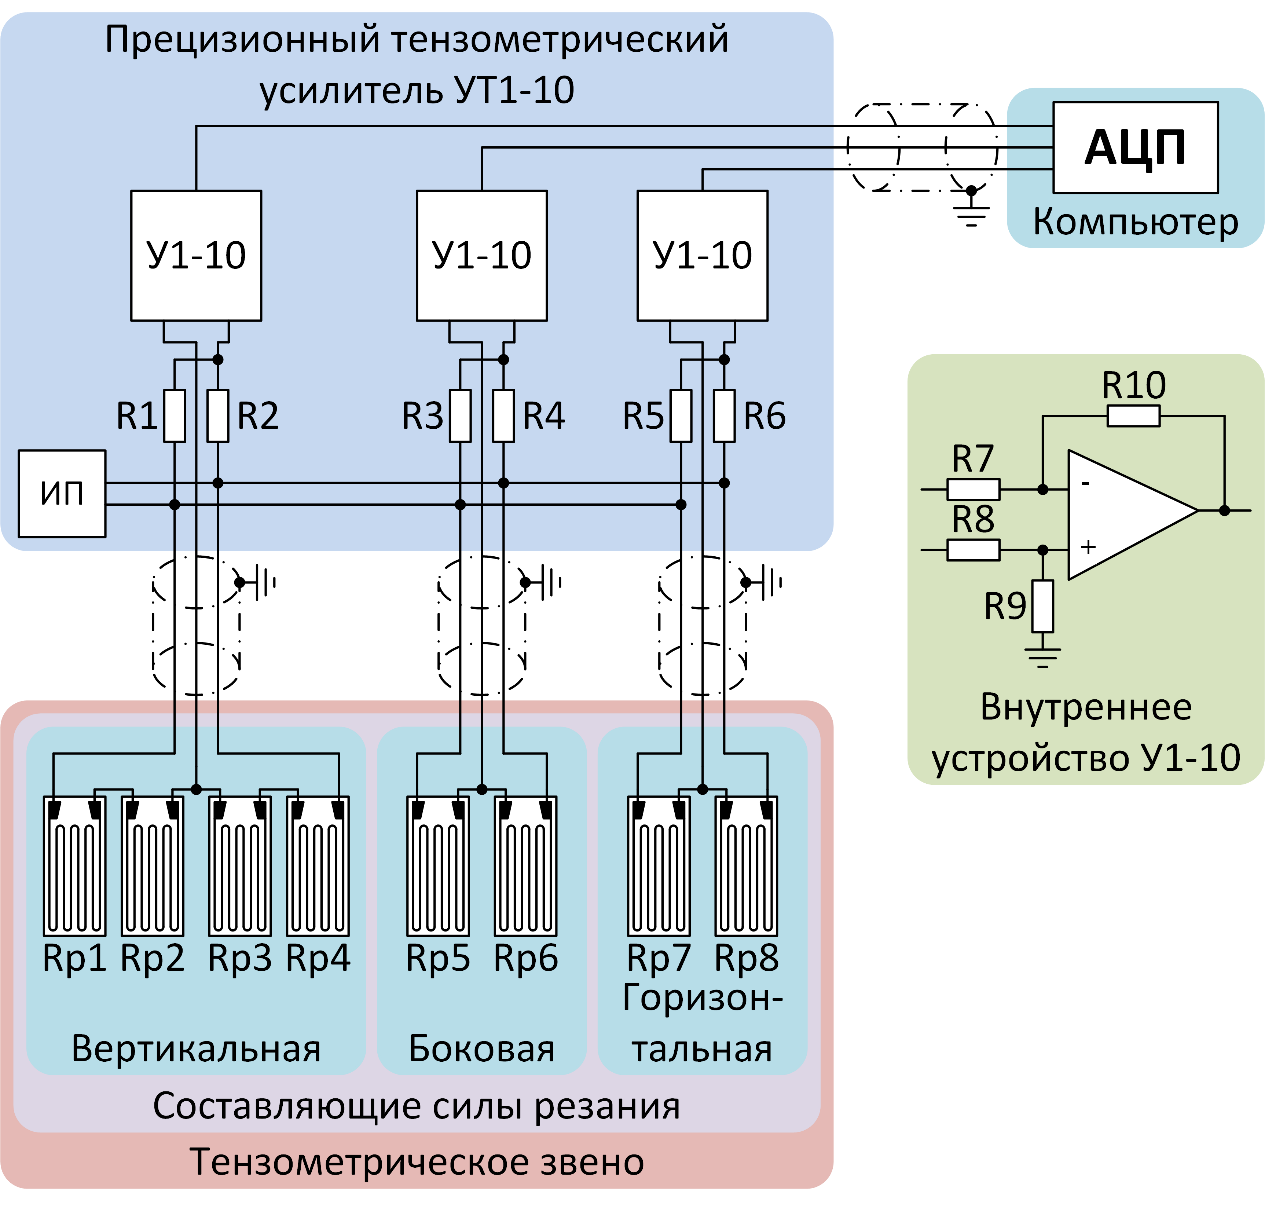
\includegraphics[width=\textwidth]{StructKomplex}
	\caption{Структурная схема измерительного комплекса для контроля силы сопротивления резанию} 
	\label{img:StructKomplex}  
\end{figure}

На рисунке \ref{img:StructKomplex} приведена структурная схема аппаратной составляющей измерительного комплекса, которая состоит из тензометрического звена, прецизионного тензометрического усилителя УТ1-10 и компьютера с установленной платой АЦП L-154. Все элементы комплекса соединены экранированным, заземлённым кабелем.

\subsection{Тензометрическое звено}\label{subsect2_4_1}

Чувствительным элементом комплекса является тензорезистор КФ5П1-20-200-А-12-С5. Имеющий следующие технические характеристики: 
\begin{itemize}
	\item номинальное электрическое сопротивление "--- $200$ Ом;
	\item ток питания "--- $20$ мА;
	\item диапазон измеряемых деформаций "--- $\pm3~000\cdot10^{-6}$;
	\item коэффициент тензочувствительности "--- $1,9\ldots2,3$ ;
	\item рабочая область температур "--- от $-$70 до $+$200~${}^\circ$С.
\end{itemize}

Тензорезистор наклеены на тензометрическое звено, представляющее собой круглую бобышку с тонкими стенками расположенную на прямоугольной плите, служащей для крепления его к лабораторному стенду. Изделие выполняется из стали марки 55С2. Такая конструкция обеспечивает наилучший уровень деформации тензорезисторов одновременно для всех составляющих силы сопротивления прочных СЛО резанию.

\begin{figure} [htbp]
	\center
	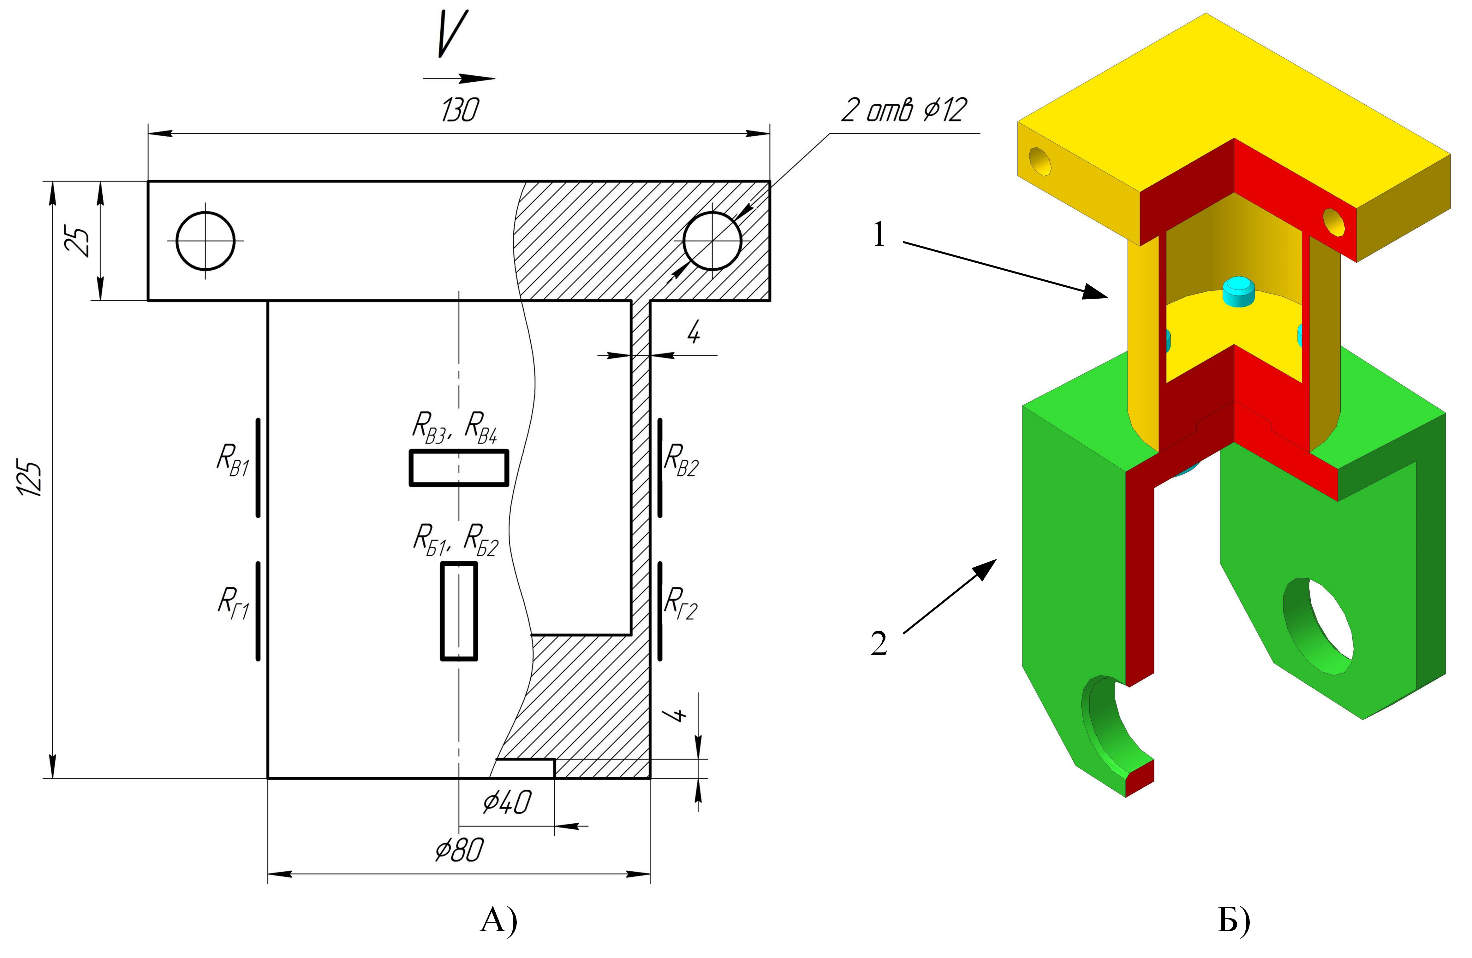
\includegraphics[width=\textwidth]{TenzoGolovka}
	
	А "--- схема наклейки тензорезисторов; Б "--- общий вид тензометрического звена;\\
	1 "--- тензометрическая головка; 2 "--- крепёж дискового режущего инструмента.
	\caption{Тензометрического звено} 
	\label{img:TenzoGolovka}  
\end{figure}

На рисунке \ref{img:TenzoGolovka} приведён общий вид тензометрического звена (Б) с установленным на него кронштейном (2) для крепления режущего инструмента. Тензометрической звено в сборе с дисковым инструментом устанавливается на лабораторный стенд описанный в \todo{[ссылки]}.

Также на рисунке \ref{img:TenzoGolovka} приведена схема наклейки тензорезисторов (А). Для измерения горизонтальной составляющей силы резания используется полу мостовая схема включения, с избирательной чувствительностью, тензорезистор $R_{\text{Г}1}$ включён в первое плечо измерительного моста, а $R_{\text{Г}2}$ – в четвёртое. Такая схема позволяет обеспечить избирательную чувствительность тензометрического моста к деформации изгиба (не чувствительна к деформации растяжения-сжатия), возникающей в следствии действия горизонтальной составляющей силы резания. Для боковой составляющей используется схема включения тензорезисторов аналогичная приведённой выше. Тензорезистор $R_{\text{Б}1}$ включён в первое плечо измерительного моста, а $R_{\text{Б}2}$ – в четвёртое. Для измерения вертикальной составляющей, диаметрально расположенные тензорезисторы $R_{\text{В}1}$ и $R_{\text{В}2}$ необходимо включить в одно плечо полумоста. Во второе плечо включаются компенсационные тензорезисторы $R_{\text{В}3}$ и $R_{\text{В}4}$, обеспечивающие также термокомпенсацию. Все схемы включения обеспечивают термокомпенсацию и компенсацию сопротивления соединительных проводов.


\subsection{Тензометрический усилитель}\label{subsect2_4_2}

Прецизионный тензометрический усилитель УТ1-10 имеет в основе прецизионный операционный усилитель (ОУ) 140УД17, двух полярный источник питания, калибровочные резисторы, стрелочные приборы указателя нулевого сигнала. ОУ имеет следующие характеристики:
\begin{itemize}
	\item максимальное выходное напряжение "--- $\pm12$ В;
	\item напряжение смещения нуля "--- $75$ мкВ;
	\item ток потребления "--- $4$ мА;
	\item коэффициент усиления напряжения – $200~000$;
	\item напряжение питания "--- $\pm(13,6\ldots16.5)$ В
	\item температура окружающей среды "--- $-$10$\ldots+$70~${}^\circ$С.;
\end{itemize}

Включение ОУ по дифференциальной схеме обеспечат исключительную чувствительность к изменению сопротивления, что в свою очередь повышает чувствительно всей системы к малому изменению нагрузки.


\subsection{Плата оцифровки сигнала}\label{subsect2_4_3}

Усиленный сигнал поступает на вход платы АЦП L-154, которая обеспечивает обработку и фиксацию сигнала в удобном для анализа виде. Плата АЦП имеет следующие характеристики:
\begin{itemize}
	\item разрядность "--- $12$ бит;
	\item диапазон входного сигнала "--- $\pm5,12$ В;
	\item максимальная частота преобразования "--- $70$ кГц;
	\item входное сопротивление "--- $2$ МОм;
\end{itemize}


\section{Тарировка тензозвена}\label{sect2_5}

Описать как проводилась тарировка, привести тарировочные графики

\section{Способ записи и хранения данных}\label{sect2_6}

Пояснить как и для чего записывать и хранить данные

\subsection{Съем данных с платы АЦП}\label{subsect2_6_1}

\subsection{Загрузка данных в MatLAB}\label{subsect2_6_2}

